%%%%%%%%%%%%%%%%%%%%%%%%%%%%%%%%%%%%%%%%%%%%%%%%%%%%%%%%%%%%%%%%%%%%%%%%
%                                                                      %
%     File: Thesis_Versat.tex                                      %
%     Tex Master: Thesis.tex                                           %
%                                                                      %
%     Author: Andre C. Marta                                           %
%     Last modified :  2 Jul 2015                                      %
%                                                                      %
%%%%%%%%%%%%%%%%%%%%%%%%%%%%%%%%%%%%%%%%%%%%%%%%%%%%%%%%%%%%%%%%%%%%%%%%

\chapter{Asynchronous Sample Rate Conversion}
\label{chapter:asrc}

An ideal Asynchronous Sample Rate Converter (ASRC) is able to convert the sample
rate of an input audio signal to a desired output sample rate without
any loss of signal quality. As oppsed to a synchronous sample rate converter,
the ASRC also needs to measure the value of the input and output sample rates
continuously to compute the conversion ratio. The ideal ASRC
converts a discrete time input signal $x[n]$, sampled at a rate $F_{s1}$, to a
continuous time signal $x(t)$, with the use of a reconstruction filter. This
signal is then filtered by an anti-aliasing filter which ensures that its output
$y(t)$ has no components which would violate Nyquist's law. Signal $y(t)$ is then
converted to a discrete time signal $y[m]$, sampled at the desired output rate
$F_{s2}$~\cite{crochiere:multirate}.

A block diagram of this model is shown in Fig.~\ref{fig:classic_analog}. Note
that the reconstruction filter and anti-aliasing filters can be combined in a
single Low Pass Filter (LPF).

\begin{figure}[!htb]
  \centering
  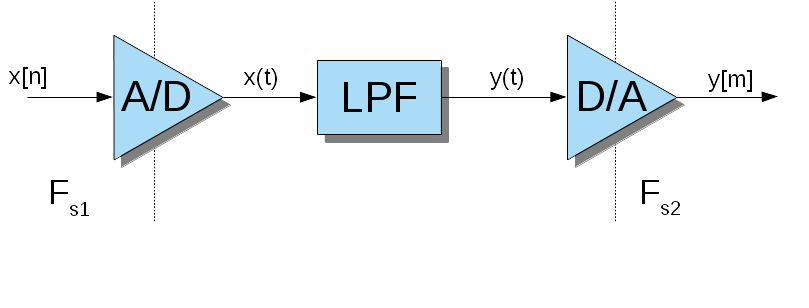
\includegraphics[width=0.8\textwidth]{Figures/classic_analog_alg.png}
  \caption{Analog interpretation of a sample rate converter}
  \label{fig:classic_analog}
\end{figure}

\section{Sample Rate Converter's Structure}
\label{section:asrc_structure}

One of the challenges of creating a purely digital solution is the design of the
LPF digital filter, which is at one time accurate and efficient.  The classical
approach to this problem consists in upsampling the signal by a factor $L$
(interpolation), doing the processing at the frequency $L \times F_{s1}$, and
downsampling the result by a factor $M$ (decimation), as a means to emulate a
discrete to continuous and continuous to discreve signal convertion~\cite{Mitra:HDSP}.
A simple block design of this algorithm is shown in Fig.~\ref{fig:classic_digital}.

\begin{figure}[!htb]
  \centering
  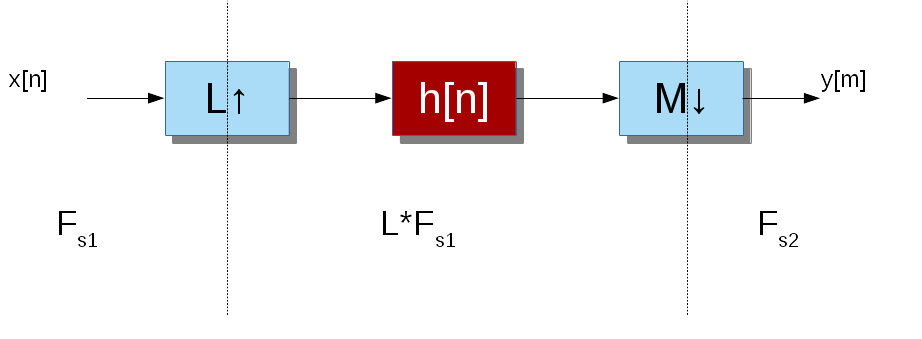
\includegraphics[width=0.8\textwidth]{Figures/classic_digital_alg.png}
  \caption{Classic digital sample rate conversion algorithm by factor L/M}
  \label{fig:classic_digital}
\end{figure}

In practice, an input signal $x[n]$, sampled at frequency $F_{s1}$ is upsampled
by insertion of $L-1$ samples with value zero between two consecutive input samples.
The resultant signal is then inserted into a low pass filter $h[n]$, which will
interpolate the inserted samples and avoid aliasing. Finally, the output of the
filter is downsampled by taking only every $M$-th sample for the output signal
$y[m]$. The relationship between $L$ and $M$ is such that

\begin{equation}
  F_{s2} = \frac{L}{M} F_{s1} .
  \label{eq:FS1_to_FS2_LM}
\end{equation}

Regarding the filter $h[n]$, its cutoff frequency depends on the relationship
described in Equation~(\ref{eq:FS1_to_FS2_LM}).  In the upsampling case ($L \geq
M$), there is the need to remove the resultant spectral images, using a filter
with a normalized cutoff frequency ($\Omega_c \leq 0.5\pi/L$). In the case of
downsampling ($L < M$), there is the need to filter signal frequencies that
would cause aliasing, leading to a filter with a normalized cutoff frequency
($\Omega_c \leq 0.5\pi/M$).  By joining the two conditions, the resultant filter
should have a cutoff frequency

\begin{equation}
  \Omega_c = min(\frac{\pi}{2L}, \frac{\pi}{2M}) [rad] .
  \label{eq:filter_cutoff}
\end{equation}

Note that the normalization considered is in relation to the upsampled frequency:

\begin{equation}
  \Omega = \frac{2\pi f}{Lf_{s1}} [rad].
  \label{eq:freq_norm}
\end{equation}

In the current state of the art, this algorithm is the basis of most synchronous
and asynchronous sample rate converters.

For conversions which use small values of $L$ and $M$ the computational effort is
modest. However, if the conversion involves sampling rates with a small
difference, the factors $L$ and $M$ will increase significantly, increasing
drastically the computational cost of the conversion, only to have most of the
computed samples discarded. Note that in this case a small normalized cutoff
frequency must be used for the filter.

Furthermore, there is the need to design the filter to both remove aliasing and
interpolate the $L-1$ inserted samples. This is why design of the filter $h[n]$
is the main challenge of this architecture. The solution presented in this
thesis is based on the use of a fractional delay filter.

Additionally, for asynchronous sample rate converters, the filter is not
only time-varying, but also varies with the sample rate ratio. This means
that there is the need to define a structure that computes the ratio
and adapts the filter. For synchronous sample rate converters, the ratio
stays constant. This can lead to a predictable filter, leading to the
possibility to trade off storage space for computation time, by
precomputing a finite set of filters~\cite{ad:asrc}.

%%%%%%%%%%%%%%%%%%%%%%%%%%%%%%%%%%%%%%%%%%%%%%%%%%%%%%%%%%%%%%%%%%%%%%%%
\section{Fractional Delay Filter}
\label{section:fd_filter}

An efficient way of obtaining an interpolated value of a sample is to consider
that the output samples needed correspond to the input samples, delayed or
advanced by a certain value. Considering a discrete-time signal $y[n]$, obtained
by delaying a signal $x[n]$,

\begin{equation}
  y[n] = x[n-\tau_d] = x[n] * h_d[n],
  \label{eq:time_delay}
\end{equation}
where $\tau_d$ is the normalized delay. For continuous signals, a time shift in
the frequency domain can be expressed as a product between an input
$X(e^{j\omega})$ and a filter $H(e^{j\omega})$,

\begin{equation}
  Y(e^{j\omega}) = H(e^{j\omega}) X(e^{j\omega}),
  \label{eq:freq_delay}
\end{equation}
where

\begin{equation}
  H(e^{j\omega}) = e^{-j\omega \tau_d}.
  \label{eq:freq_delay_H}
\end{equation}

By analysis of Equation~(\ref{eq:freq_delay_H}), it is possible to note that
a delay filter is an allpass filter with unitary gain and linear phase. However
this is only the case for a continuous time domain $x(t)$ signal. For the
digital signal $x[n]$, which needs to be reconstructed and aliasing-free, a low
pass filter with a cuttoff frequency defined by Equation~(\ref{eq:filter_cutoff})
is needed. Since both the reconstruction and
anti-aliasing filters are linear systems, they can be combined together in a
single filter whose frequency response $H_d(e^{j\Omega})$ is the product of the
frequency responses of the two filters:

\begin{equation}
  H_d(e^{j\Omega}) =   
  \begin{cases}
    1, |\Omega| < \Omega_c \\
    0, otherwise
  \end{cases}
  \label{eq:fdfilter_H}
  .
\end{equation}

To obtain the impulse response of filter $h[n]$, defined in Equation~(\ref{eq:time_delay}),
the inverse discrete-time Fourrier transform (IDTFT) of $H_d(e^{j\omega})$ is
performed.

\begin{equation}
  h[n] = IDTFT(H_d(e^{j\omega})) = \frac{1}{2\pi}\int_{-\pi}^{\pi}e^{-j\Omega\tau_{d}} e^{j\Omega n} d\Omega .
  \label{eq:idtft_h}
\end{equation}

Since the integrated function is non-zero only in the interval $-[-\Omega_c,\Omega_c]$
and $e^{-j\Omega\tau_{d}} e^{j\Omega n} = e^{j\Omega  (n-\tau_{d})}$, the integral can be solved yielding

\begin{equation}
  h[n] = \frac{sin(\Omega_c (n-\tau_{d}))}{\pi (n-\tau_{d})}.
  \label{eq:h_sine}
\end{equation}

The impulse response of the filter $h[n]$ is then defined by Equation~(\ref{eq:ideal_fd}),
which is the normalized $sinc$ function.

\begin{equation}
  h[n] = \frac{\Omega_c}{\pi}sinc\bigg[\frac{\Omega_c}{\pi}(n - \tau_d)\bigg].
  \label{eq:ideal_fd}
\end{equation}

Fig.~\ref{fig:sinc} represents this function for $\tau_{d} = 0$. Note that a
variation of $\tau_{d}$ is equivalent to a translation of the figure in the $n$
(discrete time) axis. By direct observation of the figure, it is possible to
note that for integer values of $\tau_{d}$, $h[n] = 0$ for all samples except
for $n = \tau_{d}$ where $h[n] = 1$. This is the expected filter response for an
integer delay. On the other hand, for a fractional value of $\tau_{d}$, $h[n]$
is non-zero for all samples. For the ASRC algorithm, $0 \leq \tau_{d} \leq 1$,
since the objective is to use this fractional delay filter as a way to obtain an
interpolated sample using a finite number of input neighbour samples separated
by an unitary normalized delay.


\begin{figure}[!htb]
  \centering
  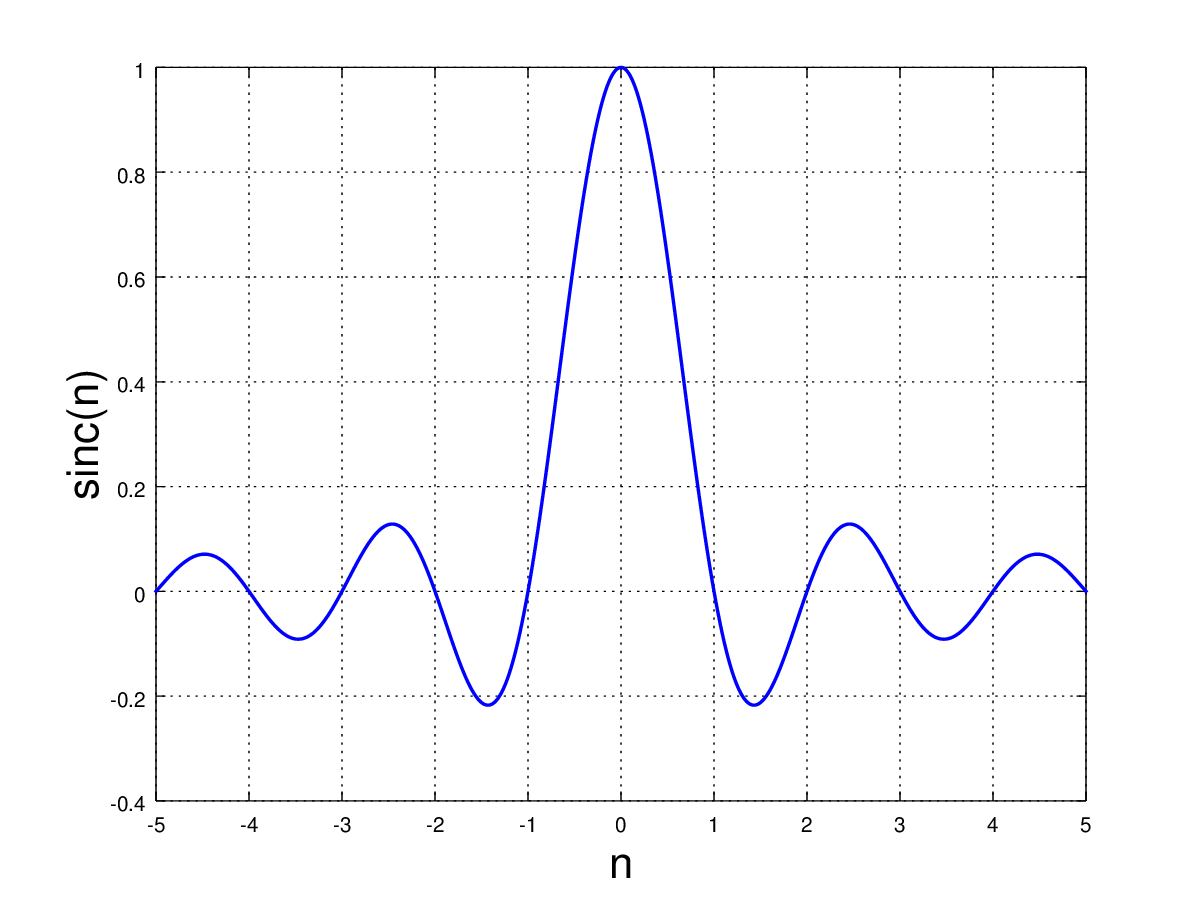
\includegraphics[width=0.8\textwidth]{Figures/sinc.png}
  \caption{Graphical representation of $h[n]$ for $\tau_{d} = 0$}
  \label{fig:sinc}
\end{figure}
  
As this function is infinite and non-causal, an approximation must be done while
retaining enough low-pass filtering capability to ensure quality, as explained
in Section~\ref{section:asrc_structure}. This
problem can be solved by applying a window to the ideal filter $h[n]$. The
choice of the format of the window and bandwidth have an influence not only on
the quality of ASRC's output signal, but also on the complexity of the
computations done.

Using the truncation of the impulse response as an approximation technique, the
resultant filter is a section of the sinc function which contains a certain
number of zeroes. To exemplify, a filter with six zeroes is considered in
Fig.~\ref{fig:exemp_upsamp}, and Fig.~\ref{fig:exemp_downsamp}.

\begin{figure}[!htb]
  \centering
  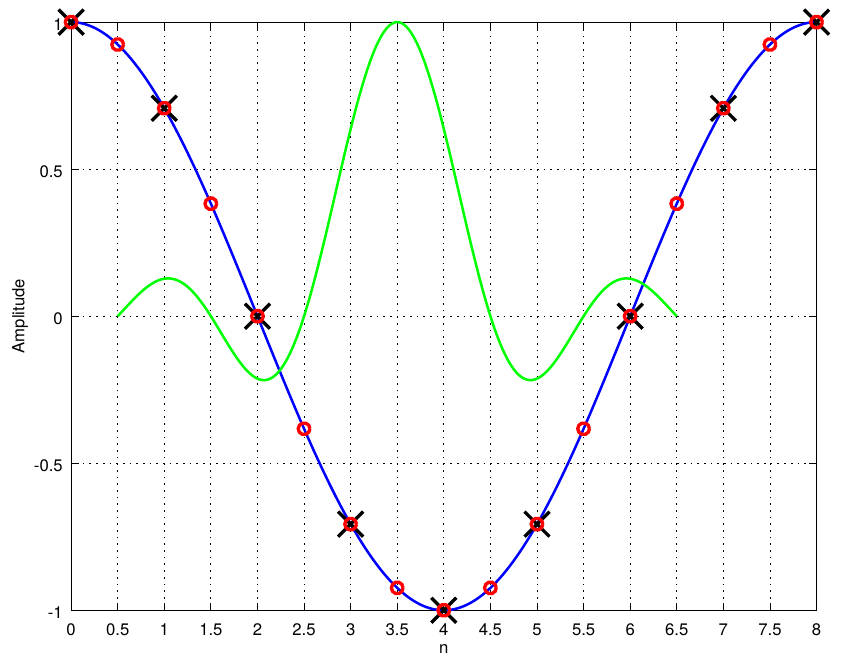
\includegraphics[width=0.8\textwidth]{Figures/upsample_example.png}
  \caption{Illustration of upsampling (1:2) used to determine the output sample
    at n = 3.5}
  \label{fig:exemp_upsamp}
\end{figure}

\begin{figure}[!htb]
  \centering
  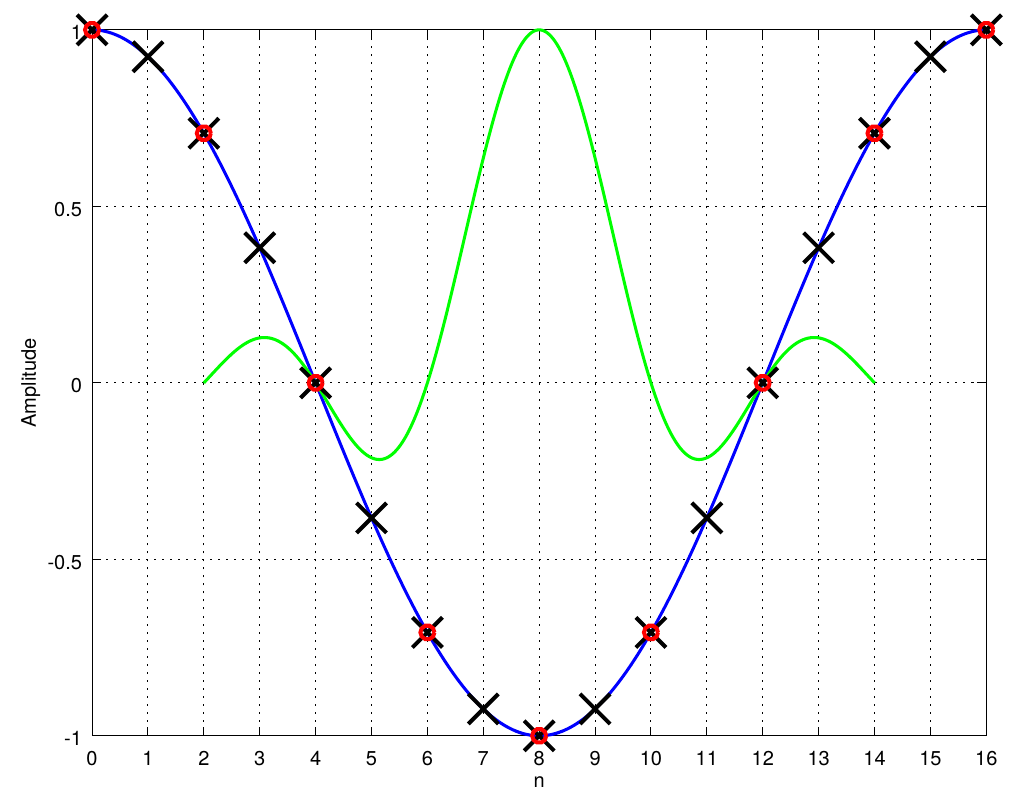
\includegraphics[width=0.8\textwidth]{Figures/downsample_example.png}
  \caption{Illustration of downsampling (2:1) used to determine the output
    sample at n = 4}
  \label{fig:exemp_downsamp}
\end{figure}


In Fig.~\ref{fig:exemp_upsamp}, the digital input signal, whose samples are
represented by crosses, is plotted along its continuous time representation. To
upsample this signal by a factor of 2, the output samples, represented by
circles, need to be computed. To interpolate these signals, the filter
approximation is applied, centring the window at the desired output sample,
multiplying each input sample by the corresponding filter value, and accumulate
all obtained values. By analysis of this illustration, it is possible to note
that a larger upsampling factor will decrease the distance between the output
samples. According to Equation~(\ref{eq:filter_cutoff}), the normalized
cutoff frequency of the filter is $0.5/L$. The filter is always the same in the
upsampling case and its number of accumulations is the same as the number of
zeroes in the truncated sinc function.

Fig.~\ref{fig:exemp_downsamp} is analogous to Fig.~\ref{fig:exemp_upsamp},
representing downsampling by a factor of 2 instead. In this case, according to
Equation~(\ref{eq:filter_cutoff}), the cutoff frequency of the filter is
given by $0.5/M$.  The number of accumulations is now $M$ times the number of
zeroes in the truncated sinc function.

Regarding the approximation of the filter itself, there is a great variety of
techniques used to obtain a fractional delay filter which minimizes the
discretization error: applying a window to the ideal filter, applying Lagrangian
interpolation to compute an intermediate coefficient from a set of known filter
samples, etc. These and other methods are explained in detail
in~\cite{kootsookos:firapproxfd,Tseng:firfdsnr,laakso:pfdfilter,Yardin:Perffdf}.


%%%%%%%%%%%%%%%%%%%%%%%%%%%%%%%%%%%%%%%%%%%%%%%%%%%%%%%%%%%%%%%5
\section{Output Sample Computation}
\label{section:output_computation}

As shown in Fig.~\ref{fig:exemp_upsamp} and \ref{fig:exemp_downsamp}, to obtain
an output sample, the fractional delay filter is applied to the input signal, by
centring it to the desired time of the output sample and computing the result of
the (discrete) convolution, as expressed in Equation~(\ref{eq:time_delay}).
Furthermore, it is important to note that, since this converter is applied to
audio, the digital design of the filter should make sure that the filter has
linear phase. This is achieved by using a Finite Impulse Response (FIR), which
has a non-recursive structure. In an FIR, each output $y[n]$ is obtained by

\begin{equation}
  y[n] = \sum_{i=0}^N a_i x[n-i],
  \label{eq:macc}
\end{equation}

where $a_i$ are the coefficients of the filter and $x[n-i]$ is the input sample
at discrete time $n-i$. It is important to note that the filter described in
Section~\ref{section:fd_filter} is non causal. To fix this, the computation of
the output is delayed by as many input samples as accumulations that involve
future input samples.

With this implementation, the computation of an output sample is reduced to a
multiply-accumulate (macc) operation. However, it requires a large amount of
filter coefficients, which, in hardware, results in high memory usage, an
undesirable result.

To guarantee that the sample rate converter supports multiple
channels, the structure of the converter should be able to support the computation
of multiple output samples. This can be done at the cost of hardware area,
by having one output computation unit per channel, or at the cost of computation
time, by having one unit computing multiple outputs sequentially. To make
this possible, there is the need to optimize this not only regarding hardware
area, but also computation time.

\section{Sample Rate Converter Implementations: An Analysis Of The State Of The Art}
\label{section:implementation}

\subsection{Cascaded Integrator Comb Filters (CIC)}

As was explained in Section~\ref{section:asrc_structure}, sample rate conversion
can be interpreted as signal upsampling with interpolation, followed by
downsampling with decimation. Furthermore, this algorithm can be implemented
using FIR filters as shown in the previous section. One of the designs comonly
used for this purpose is a Cascaded Integrator Comb filter
(CIC)~\cite{charanjit:impl}. This filter, originally designed by Hogenauer~\cite{hogenauer},
is based on the implementation of simple integrators and
differentiators.  CIC filters are obtained by combining adders and delay
registers, which consumes a reduced amount of memory and has the great advantage
of dispensing with multipliers, which can consume a great amount of hardware
resources. Due to the fact that the CIC decimator has a symetric structure in
comparinson to a CIC interpolator, the combination of the two components leads
to a highly efficient implementation in application specific integrated circuits
(ASIC) and FPGA's. An interpolation filter using the CIC structure can be seen
in Fig.~\ref{fig:cic_basic}. A decimation filter would have the same components,
with the difference that the comb filters and integrator stages would swap
positions.

\begin{figure}[!htb]
  \centering
  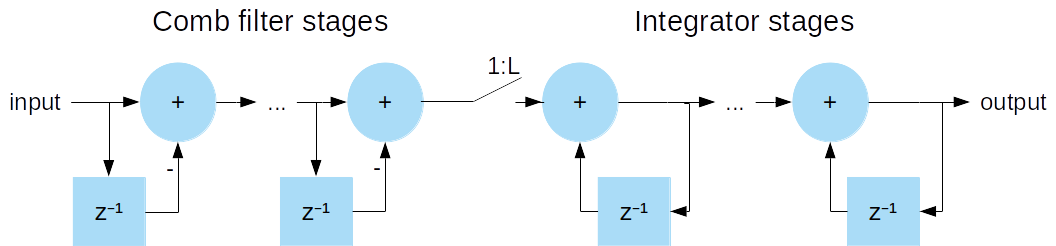
\includegraphics[width=\textwidth]{Figures/cic_filter.png}
  \caption{Example of cascaded integrator comb filter structure, used as an interpolation filter}
  \label{fig:cic_basic}
\end{figure}

While for one CIC structure, the frequency response does not fulfill the
requirements, this problem can be solved by cascating multiple interpolation and
integration units \cite{charanjit:impl}, increasing the attenuation in the
filter's stopband. This implementation is elegant but has limited
configurability, due to the fact that no coefficients are used, making it hard
to adapt the filter to variations in the sample rates. Furthermore, this type of
filter expects integer factors, which leads to the problem of making it able to
convert fractional sample rate relations.

\subsection{Approximation By Piecewise Quadratic Function}
\label{subsection:piecewise}

As explained in Section~\ref{section:fd_filter}, a direct way to implement the
sample rate converter is to consider that the algorithm can be reduced to simply
applying a fractional delay filter to the input signal, with a sinc impulse
response as expressed by Equation~(\ref{eq:ideal_fd}). In practice this is
impossible because the filter has an infinite number of taps and requires the
use of future samples (non-causality).

The solution presented so far is to truncate and approximate the coefficients
and delay the response to make it causal. Another way to address this problem is
to split the sinc function into a piecewise function, and aproximate each piece
by a quadractic function, leading to an interpolation filter which can be easily
implemented~\cite{aikawa:kernel,aikawa:kernel_hw}. The approximation of the
piecewise sinc function $h(x)$ into quadractic functions can be expressed as

\begin{equation}
	h(t) = 
	\begin{cases}
		a_{1,1}t^2+b_{1,1}t + c_{1,1}, \bigg(0 \leq |t| \leq \frac{1}{N}\bigg)\\
		\vdots \\
		a_{1,n}t^2+b_{1,n}t + c_{1,n}, \bigg(\frac{n-1}{N} \leq |t| \leq 1\bigg)\\
		\vdots \\
		a_{s,n}t^2+b_{s,n}t + c_{s,n}, \bigg(s-1+\frac{n-1}{N} \leq |t| \leq s-1+\frac{n}{N}\bigg)\\
		\vdots \\
		a_{S,n}t^2+b_{S,n}t + c_{S,n}, \bigg(S-1+\frac{n-1}{N} \leq |t| \leq S\bigg)
	\end{cases}
,
	\label{eq:kernel}
\end{equation}
where $N$ is the number of quadratic functions used to represent a piecewise
function, and $S$ is the number of piecewise functions of the kernel. This
technique leads to the implementation presented in Fig. \ref{fig:kernel}.

\begin{figure}[!htb]
  \centering
  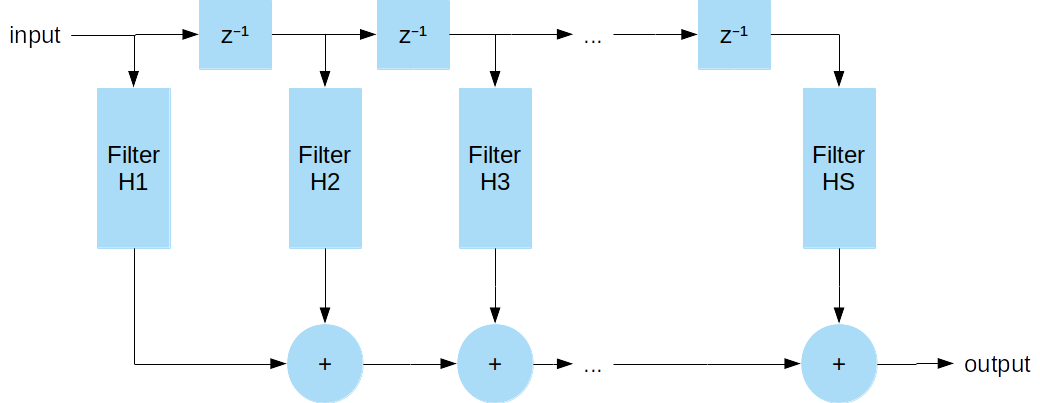
\includegraphics[width=\textwidth]{Figures/kernel_filter.png}
  \caption{Example of a piecewise kernel filter structure}
  \label{fig:kernel}
\end{figure}

This design can be futher optimized, by considering that from a certain section
onward, the polynomial remains the same, changing only in scale by a determined
set of factors $e_j$. The block diagram of this structure is presented in
Fig.~\ref{fig:kernel_block}. This leads to a structure where the polynomials
used remain the same, while the factors $e_j$ change with the sample rate
convertion ratio. There are, however, some restrictions that need to be
considered, as further explained in~\cite{aikawa:kernel}.

\begin{figure}[!htb]
  \centering
  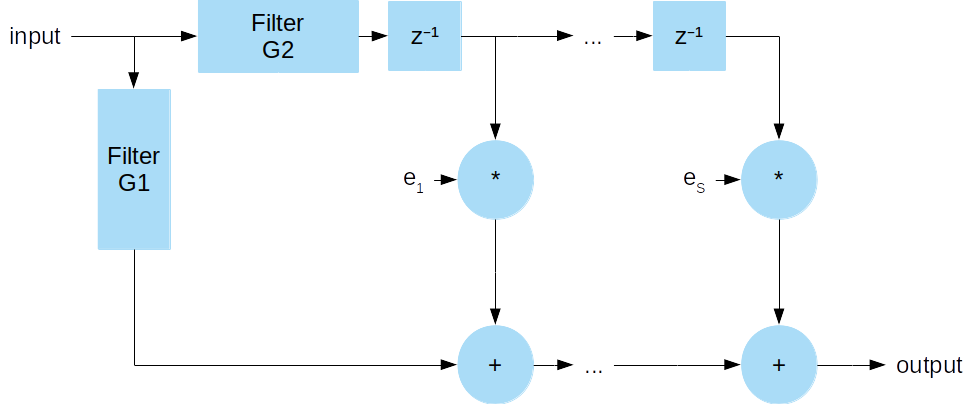
\includegraphics[width=\textwidth]{Figures/kernel_filter_2.png}
  \caption{Example of optimized kernel filter structure}
  \label{fig:kernel_block}
\end{figure}

The main advantage of this design is the ability to change sample rate ratio
without need to reconfigure the filter, leading to a kernel which not only is
able to implement the function, but also does not need to change over
time. However, as one needs to define a high number of pieces to obtain large
attenuation in the stopband (to acceptably attenuate distortion and noise), it
is needed to use a large number of quadratic functions, which significantly
increases the computational cost. Apart from the structure itself, there is
still the high cost of computing the coefficients $e_j$, which turns even more
problematic with applications for which the sample rate convertion ratio varies
in time.

\subsection{Farrow Structure}

The most common implementations of fractional delay filters, and, by
consequence, sample rate converters, is one which uses the Farrow Structure
\cite{Farrow:farrow_structure}.  This structure is based on the assumption that
each sample of the filter impulse response $h[n]$ can be approximated by a
polynomial of order $q$, which depends on the fractional delay
$d$~\cite{Blok:VariableRS}:

\begin{equation}
	h[n] = \sum_{m=0}^{q} c_m[n]d^m.
	\label{eq:farrow_approx}
\end{equation}

Similar to the structure presented in Section~\ref{subsection:piecewise}, a
Farrow structure requires the implementation of a set of $q$ FIR filters, which
becomes a hardware-intensive design. Furthermore, a change in the fractional
delay forces the change of all coefficients, leading to an increase of the
computational cost. Over the years, this structure has been subjected to many
changes and optimizations, with the objective to develop filters for different
applications. For the specific application this thesis is concerned, the
structure is optimized to design filters with a variable fractional delay.  One
possible optimization, further explained in~\cite{babic:farrow_optimization},
makes it possible to implement a low area Farrow structure, with the great
advantage of having fixed coefficients and a single parameter $\mu$ that depends
on the fractional delay. The block design of this structure is presented in
Fig.~\ref{fig:farrow_structure}, where the value of $\mu$ can be computed by

\begin{figure}[!htb]
  \centering
  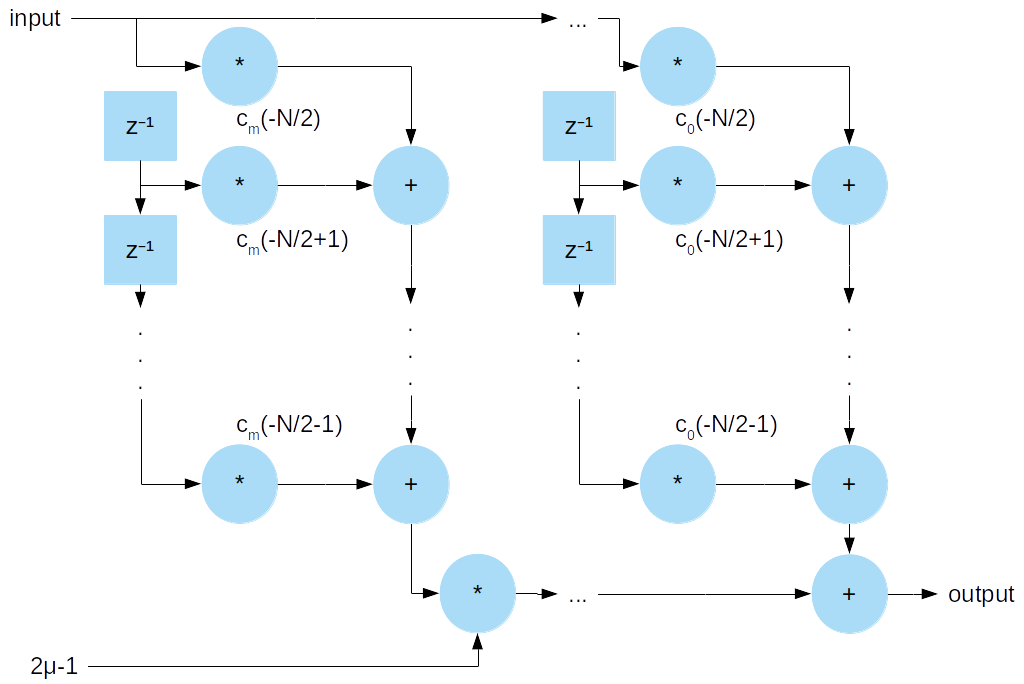
\includegraphics[width=\textwidth]{Figures/farrow_struct.png}
  \caption{Example of farrow structure, optimized for variable fractinal delay}
  \label{fig:farrow_structure}
\end{figure}


\begin{equation}
	\mu = \frac{k}{M},
	\label{eq:mu_farrow}
\end{equation}
where $M$ is the decimation factor and $k \in \{0,1,2,...\}$, is a value which
increments throughout the computation of the output. The transfer function of
each FIR subfilter, $C_m (z)$ is expressed by

\begin{equation}
	C_m (z) = \sum_{k=0}^{N-1}c_m \bigg(k-\frac{N}{2}\bigg)z^{-k} .
	\label{eq:farrow_sub_transferfunc}
\end{equation}

While the structure presented in Fig.~\ref{fig:farrow_structure} is optimized
for interpolation, there are some modifications, explained in detail
in~\cite{babic:farrow_optimization} which apply to decimation. This structure has
the disadvantage of having to include all subfilters to compute all coefficients
$c_n$, it is one of the easiest methods to allow variations on sample rate
conversion ratios, and occupies a low area, which is mainly taken by the delay
elements.
